\section{Results}
\label{sec:results}

Figure \ref{fig:main_result} shows the results from the experiments. Figure \ref{fig:original_result} shows the results from the original paper. This section examines the results from this project and compares them to the original. 

\begin{figure}[H]
    \centering
    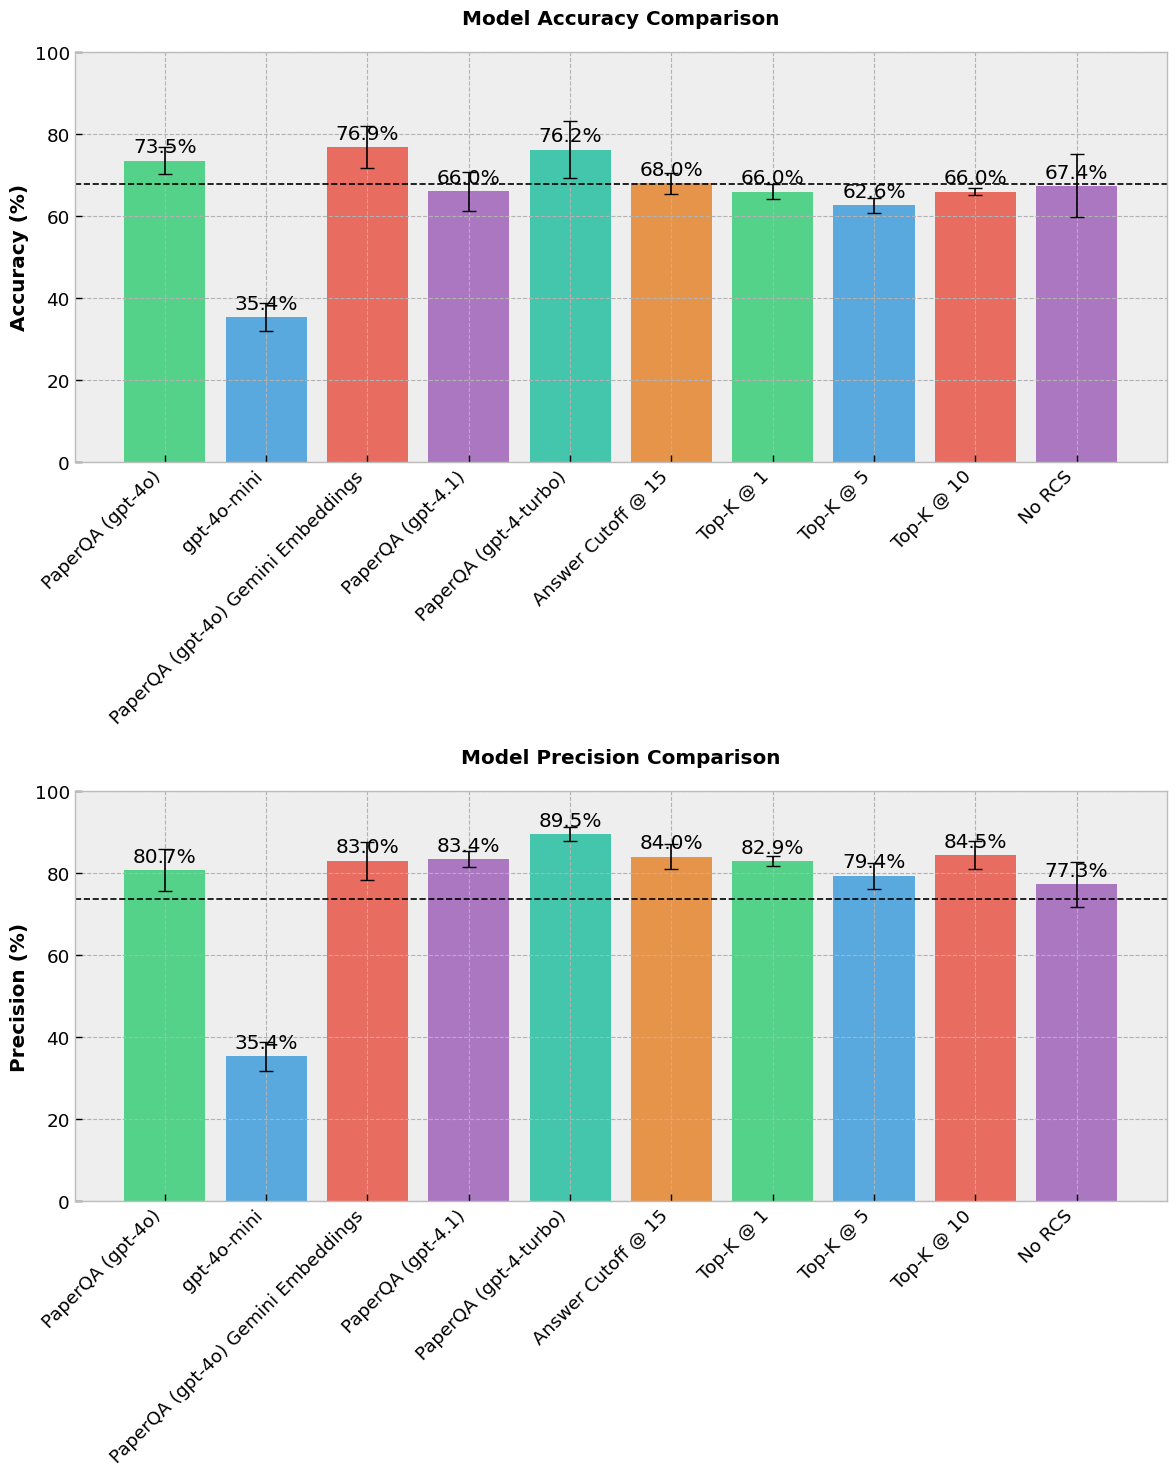
\includegraphics[width=\textwidth]{figures/main_result.png}
    \caption{This project's results against the LitQA test set. Top: Average accuracy of various setups of PaperQA. Bottom: Average precision of the various setups of PaperQA.}
    \label{fig:main_result}
\end{figure}

\begin{figure}[H]
    \centering
    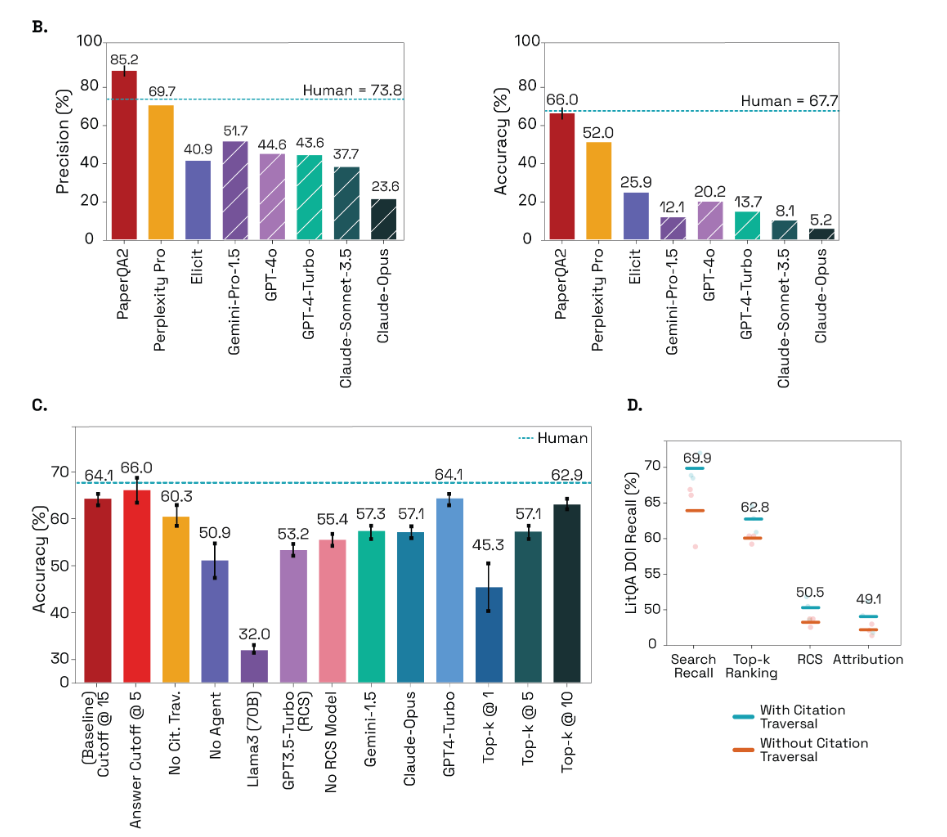
\includegraphics[width=\textwidth]{figures/original_result.png}
    \caption{Original Paper Results. B: Precision and Accuracy of PaperQA and LLMs on LitQA. C: Accuracy of verious abalations of PaperQA. D: Aggragated DOI Recall at each stage (This result is not relevant to this report.)}
    \label{fig:original_result}
\end{figure}

\subsection{RAG vs. Standalone LLM}

SIMILAR TO ORIGINAL: PAPERQA outperforms SINGLE LLMS. 

HOWEVER GPT MINI ATTEMPTS TO ASNWER ALL QUESTIONS HENCE SAME ACC AND PREC, THIS DOES NOT HAPPEN FOR THE SINGLE LLM RESULTS IN ORIGINAL PAPER. 


\subsection{PaperQA Ablations}
OUR BASELINE is Top-k of 30. Asnwer Cutoff at 5, and it is the PaperQA (gpt-4o-mini). 

Comparing their baseline to our gpt4-turbo result, it is fairly similar. But we have a much bigger spread. 

Gpt -4 turbo result seems errorneous. Very large spread and outperforms newer and better performing models. 

Gemini embedding has best result. 

Reducing top k reduces accuracy. HAS A MUCH BIGGER EFFECT THAN IN PAPER. ALSO TREND IS REVERSED COMPARED TO PAPER. 

Increasing Answer Cutoff decreases accuracy. SAME TREND AS ORIGINAL PAPER. 

Precision is simialr across the ablations. RAG performs much better than non-RAG. 

RCS decreases accuracy and precision but has less of an effect than reducing top k for accuracy. 





